\chapter{Anexo I} 	% Main chapter title
\label{AppendixA} 	% nao pode ser em capítulo tem de ser em apêndice
%%%%%%%%%%%%%%%%%%%%%%%%%%%%%%%%%%%%


\section{Query}
\label{sec:query}
\textbf{Query}: ("urban logistics*" OR "urban areas*") AND ("smart cities*" OR "city logistics*" OR "smart logistics*") AND (sustainab* OR efficien* OR innovat*) AND ("transportation*" OR "economics*" OR "management*").

\section{\gls{wos} Web of Science Results}
\label{sec:wos_results}
A \gls{fig} abaixo analisa os resultados obtidos com a query acima no \gls{wos}.
\begin{figure}[H]
    \centering
    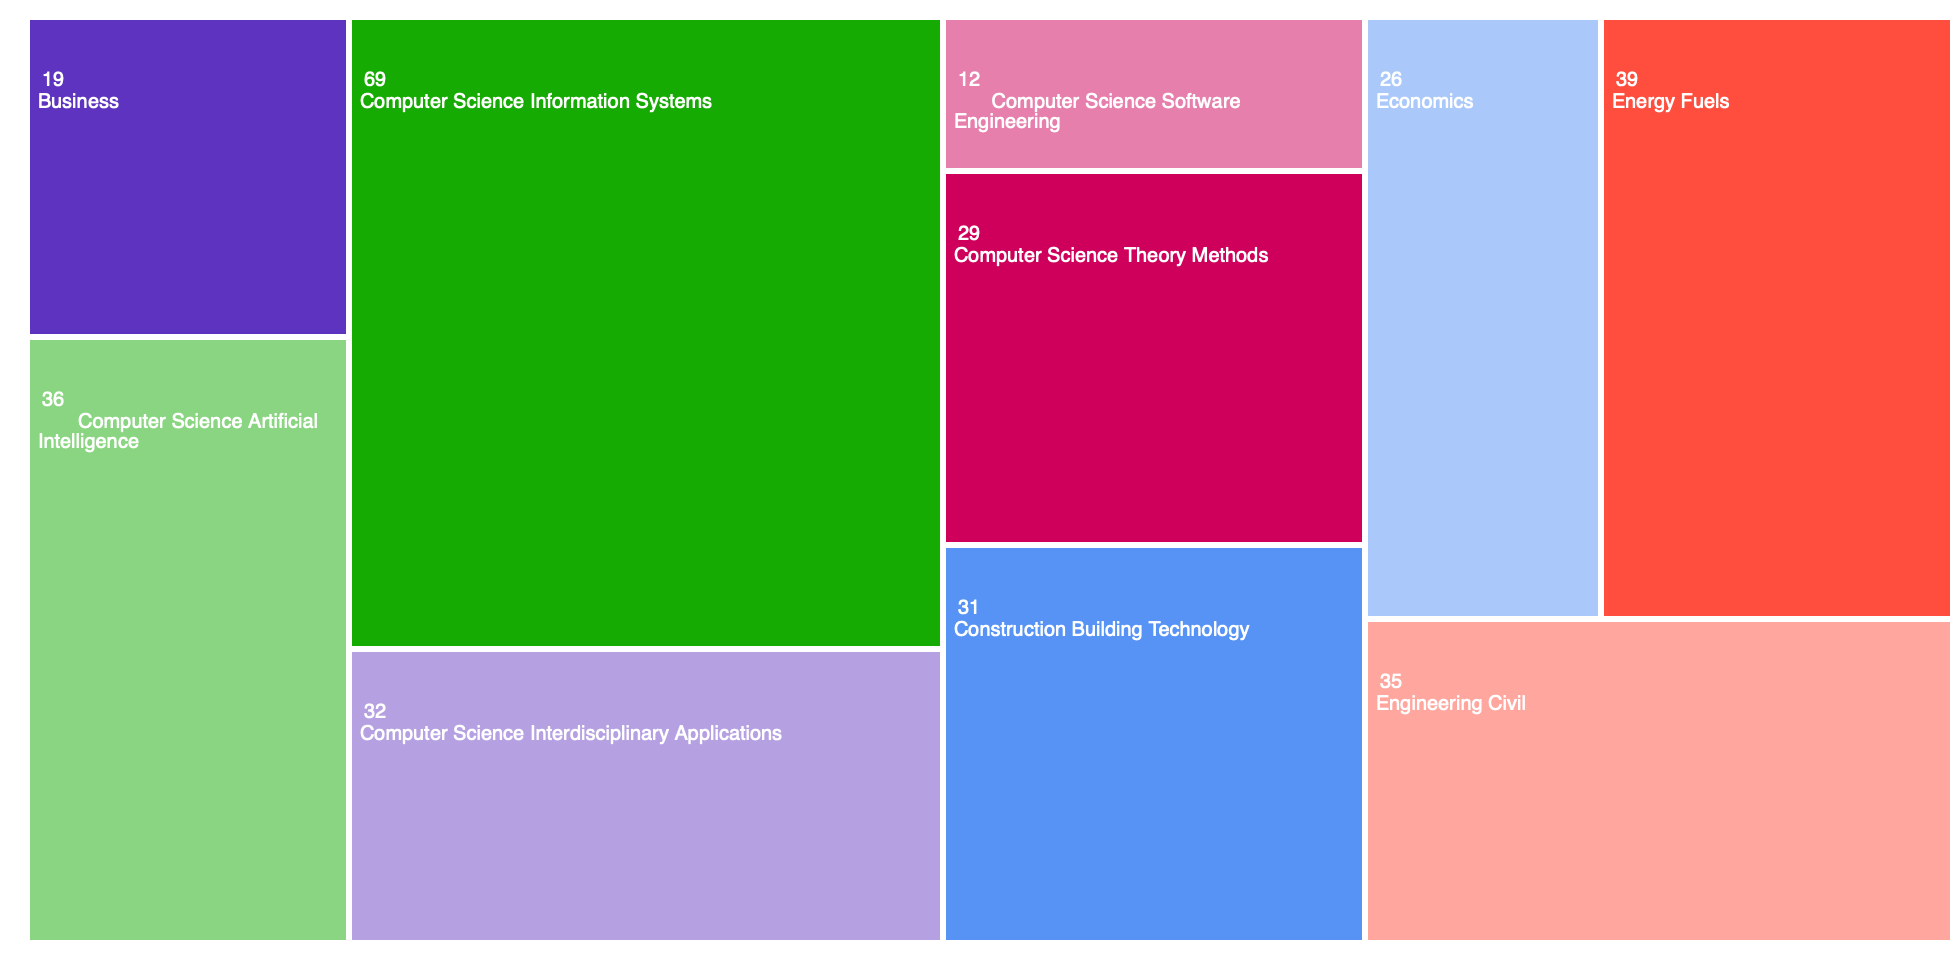
\includegraphics[width=0.99\textwidth]{figures/appendixA/visualization-web-of-science-category.jpg}
    \caption{Resultados das Categorias das áreas de estudo obtidas no \gls{wos} com a query definida.}
    \label{fig:wos_query_results}
\end{figure}    

A \gls{fig} abaixo agora analisa os anos de publicação dos artigos obtidos com a query acima no \gls{wos}.

\begin{figure}[H]
    \centering
    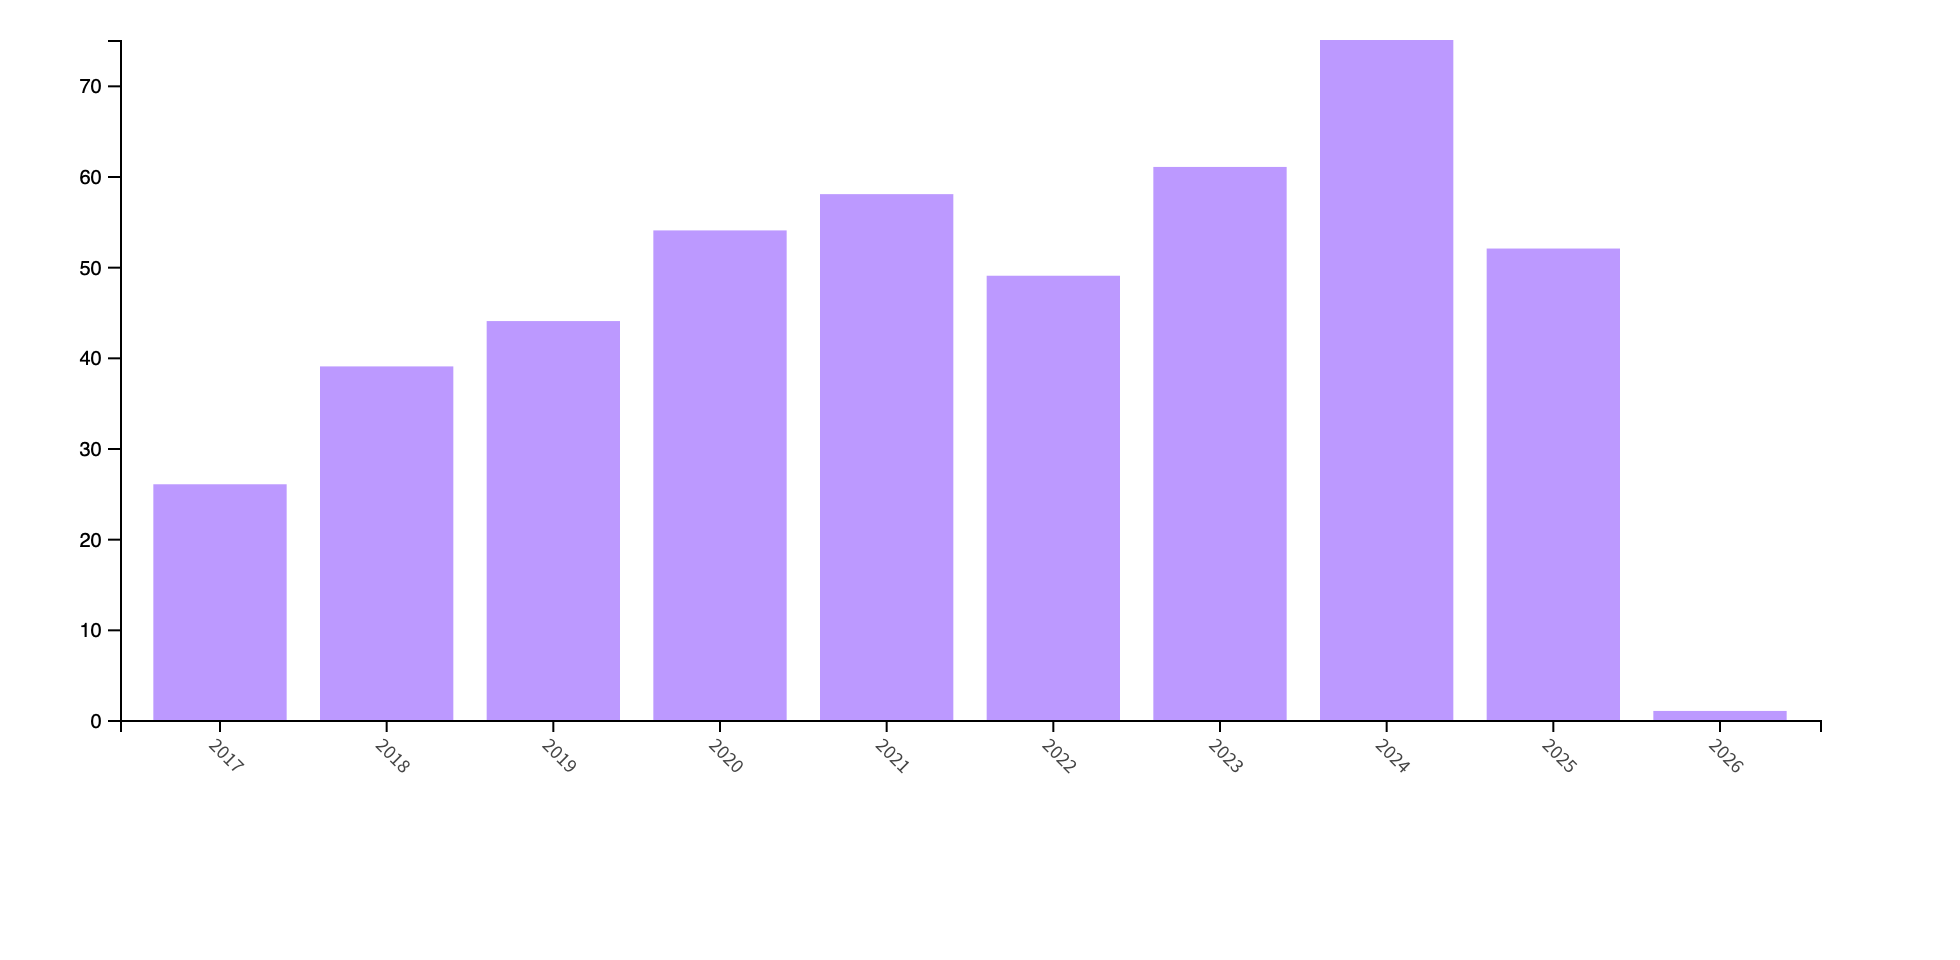
\includegraphics[width=0.99\textwidth]{figures/appendixA/visualizationpublication-years.jpg}
    \caption{Resultados dos Anos de Publicação dos artigos obtidos no \gls{wos} com a query definida.}
    \label{fig:wos_query_years}
\end{figure}

\section{\gls{vosviewer} Visualizations}
\label{sec:vosviewer_visualizations}

A \gls{fig} abaixo apresenta a visualização de rede obtida com a ferramenta \gls{vosviewer} com base nos 536 artigos obtidos no \gls{wos} com a query definida.
\begin{figure}[H]
    \centering
    %\includegraphics[width=0.99\textwidth]{figures/appendixA/visualization-vosviewer-network.jpg}
    %\caption{Visualização de Rede obtida com a ferramenta \gls{vosviewer} com base nos 536 artigos obtidos no \gls{wos} com a querydefinida.}
    \label{fig:vosviewer_network}
\end{figure}

A \gls{fig} abaixo apresenta a visualização de densidade obtida com a ferramenta \gls{vosviewer} com base nos 536 artigos obtidos no \gls{wos} com a query definida.
\begin{figure}[H]
    \centering
    %\includegraphics[width=0.99\textwidth]{figures/appendixA/visualization-vosviewer-density.jpg}
    %\caption{Visualização de Densidade obtida com a ferramenta \gls{vosviewer} com base nos 536 artigos obtidos no \gls{wos} coma query definida.}
    \label{fig:vosviewer_density}
\end{figure}

\section{Repositório \gls{github}}
\label{sec:github_repository}
O repositório público do \gls{github} onde a informação foi guardada e sequencialmente atualizada ao longo de todo o trabalho está disponível em: \url{https://
github.com/JunqueiraDev/Eduardo-Urban-Logistics-in-Smart-Cities}.
Como existe uma diferença, de dois anos, existe um lapso de que no  ano passado 2025 existia -536 resultados  e que, este ano, 2026 existem apenas 533 artigos, a informação da ferramenta destes dados é o \gls{wos} que pode variar futuramente. Assim, o repositório do \gls{github} serve de consultada da data até ao momento que foi obtido os dados \cite{JunqueiraDevEduardoRepositório}.
